\documentclass{report}

\usepackage{listings}
\usepackage{polski}
\usepackage[utf8]{inputenc}
\usepackage[margin=1in]{geometry}
\usepackage[english,polish]{babel}\usepackage{indentfirst}
\usepackage[T1]{fontenc}
\usepackage{xcolor}
\usepackage{graphicx}
\usepackage{longtable}

\pagecolor{black}
\color{white}

\begin{document}
    \tableofcontents

    \chapter{Wstęp}

    \section{Cel projektu}

    \section{Motywacja}

    \chapter{Problem medyczny}

    Wybrany przeze mnie problem medyczny dotyczy klasyfikacji stanów ostrego brzucha.
    Za ten stan odpowiedzialne mogą być różne choroby, które zawsze wymagają interwejcji lekarza.
    % http://www.poradnikzdrowie.pl/zdrowie/uklad-pokarmowy/ostry-brzuch-przyczyny-objawy-leczenie-ostrego-brzucha_35445.html

    \section{Opis chorób}

    Do klasyfikacji jest 8 chorób, zatem sieć neuronowa będzie miała za zadanie przypisać 1 z 8 klas.
    Są to:
    \begin{enumerate}
        \item Ostre zapalenie wyrostka robaczkowego
        \item Zapalenie uchyłków jelit
        \item Niedrożność mechaniczna jelit
        \item Perforowany wrzód trawienny
        \item Zapalenie woreczka żółciowego
        \item Ostre zapalenie trzustki
        \item Niecharakterystyczny ból brzucha
        \item Inne przyczyny ostrego bólu brzucha
    \end{enumerate}

    \begin{figure}[h!]
        \centering
        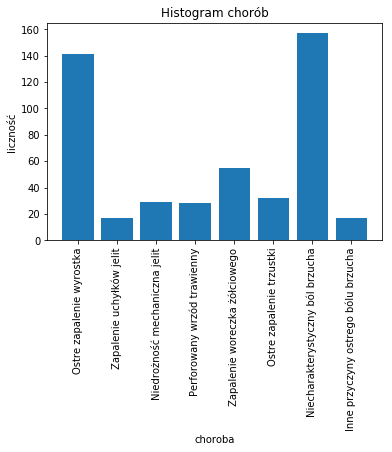
\includegraphics[scale=0.7]{./img/histogram.png}
        \caption{Histogram występowania chorób}
        %        \label{}
    \end{figure}

    Histogram pokazuje, że rozkład klas jest nierównomierny.
    Na 476 obiektów aż 157 to 'Niecharakterystyczny ból brzucha' i 141 ma etykietę 'Ostre zapalenie wyrostka robaczkowego'.
    Czyli do 2 klas należy ponad 60\% obiektów.
    Może to mieć negatywny wpływ na jakość klasyfikacji.

    \section{Opis cech}

    Dane do tego problemu zawierają 31 cech.
    Są to odpowiedzi z wywiadu medycznego i wyniki przeprowadzonych badań.
    Możliwe wartości parametrów przedstawione są poniżej.
    Jak widać wszystkie liczby są naturalne mniejsze niż 11, także normalizacja czy skalowanie danych nie jest konieczne.

    
\begin{longtable}{|c|l|l|}
    \caption{Wszystkie cechy z odpowiedziami}\\ \hline
    \textbf{L.p.} & \textbf{Pytanie} & \textbf{Możliwe odpowiedzi} \\ \hline
    \endfirsthead
    \multicolumn{3}{c}
    {\tablename\ \thetable\ -- \textit{Wszystkie cechy z odpowiedziami - c.d.}} \\ \hline
    \textbf{L.p.} & \textbf{Pytanie} & \textbf{Możliwe odpowiedzi} \\ \hline
    \endhead
    \hline \multicolumn{3}{r}{\textit{Kontynuacja na następnej stronie}} \\
    \endfoot
    \hline
    \endlastfoot

\multicolumn{3}{|c|}{Ogólne} \\ \hline
1 & Płeć & \begin{tabular}[c]{l}1) męska  \\ 2) żeńska \end{tabular} \\ \hline
2 & Wiek & \begin{tabular}[c]{l}1) poniżej 20 lat  \\ 2) 20 - 30 lat  \\ 3) 21 - 30 lat  \\ 4) 31 - 40 lat  \\ 5) 41 - 50 lat  \\ 6) powyżej 50 lat \end{tabular} \\ \hline
\multicolumn{3}{|c|}{Ból} \\ \hline
3 & Lokalizacja bólu na początku zachorowania & \begin{tabular}[c]{l}1) prawa górna ćwiartka  \\ 2) lewa górna ćwiartka  \\ 3) górna połowa  \\ 4) prawa połowa  \\ 5) lewa połowa  \\ 6) centralny kwadrat  \\ 7) cały brzuch  \\ 8) prawa dolna ćwiartka  \\ 9) lewa dolna ćwiartka  \\ 10) dolna połowa \end{tabular} \\ \hline
4 & Lokalizacja bólu obecnie & \begin{tabular}[c]{l}0) brak bólu  \\ 1) prawa górna ćwiartka  \\ 2) lewa górna ćwiartka  \\ 3) górna połowa  \\ 4) prawa połowa  \\ 5) lewa połowa  \\ 6) centralny kwadrat  \\ 7) cały brzuch  \\ 8) prawa dolna ćwiartka  \\ 9) lewa dolna ćwiartka  \\ 10) dolna połowa \end{tabular} \\ \hline
5 & Intensywność bólu & \begin{tabular}[c]{l}0) łagodny/brak  \\ 1) umiarkowany  \\ 2) silny \end{tabular} \\ \hline
6 & Czynniki nasilające ból & \begin{tabular}[c]{l}0) brak czynników  \\ 1) oddychanie  \\ 2) kaszel  \\ 3) ruchy ciała \end{tabular} \\ \hline
7 & Czynniki przynoszące ulgę & \begin{tabular}[c]{l}0) brak czynników  \\ 1) wymioty  \\ 2) pozycja ciała \end{tabular} \\ \hline
8 & Progresja bólu & \begin{tabular}[c]{l}1) ustepujący  \\ 2) bez zmian  \\ 3) nasilający się \end{tabular} \\ \hline
9 & Czas trwania bólu & \begin{tabular}[c]{l}1) mniej niż 12 godzin  \\ 2) 12 - 24 godzin  \\ 3) 24 - 48 godzin  \\ 4) powyżej 48 godzin \end{tabular} \\ \hline
10 & Charakter bólu na początku zachorowania & \begin{tabular}[c]{l}1) przerywany  \\ 2) stały  \\ 3) kolkowy \end{tabular} \\ \hline
11 & Charakter bólu obecnie & \begin{tabular}[c]{l}0) brak bólu  \\ 1) przerywany  \\ 2) stały  \\ 3) kolkowy \end{tabular} \\ \hline
\multicolumn{3}{|c|}{Inne objawy} \\ \hline
12 & Nudności i wymioty & \begin{tabular}[c]{l}0) brak  \\ 1) nudności bez wymiotów  \\ 2) nudności z wymiotami \end{tabular} \\ \hline
13 & Apetyt & \begin{tabular}[c]{l}1) zmniejszony  \\ 2) normalny  \\ 3) zwiększony \end{tabular} \\ \hline
14 & Wypróżnienia & \begin{tabular}[c]{l}1) biegunki  \\ 2) prawidłowe  \\ 3) zaparcia \end{tabular} \\ \hline
15 & Oddawanie moczu & \begin{tabular}[c]{l}1) normalne  \\ 2) dysuria \end{tabular} \\ \hline
\multicolumn{3}{|c|}{Historia} \\ \hline
16 & Poprzednie niestrawności & \begin{tabular}[c]{l}0) nie  \\ 1) tak \end{tabular} \\ \hline
17 & Żółtaczka w przeszłości & \begin{tabular}[c]{l}0) nie  \\ 1) tak \end{tabular} \\ \hline
18 & Poprzednie operacje brzuszne & \begin{tabular}[c]{l}0) nie  \\ 1) tak \end{tabular} \\ \hline
19 & Leki & \begin{tabular}[c]{l}0) nie  \\ 1) tak \end{tabular} \\ \hline
\multicolumn{3}{|c|}{Ogólne badanie} \\ \hline
20 & Stan psychiczny & \begin{tabular}[c]{l}1) pobudzony/cierpiący  \\ 2) prawidłowy  \\ 3) apatyczny \end{tabular} \\ \hline
21 & Skóra & \begin{tabular}[c]{l}1) blada  \\ 2) prawidłowa  \\ 3) zaczerwieniona (twarz) \end{tabular} \\ \hline
22 & Temperatura (pacha) & \begin{tabular}[c]{l}1) poniżej 36.5 stC  \\ 2) 36.5 - 37 stC  \\ 3) 37 - 37.5 stC  \\ 4) 37.5 - 38 stC  \\ 5) 38 - 39 stC  \\ 6) powyżej 39 stC \end{tabular} \\ \hline
23 & Tętno & \begin{tabular}[c]{l}1) poniżej 60 /min  \\ 2) 60 - 70 /min  \\ 3) 70 - 80 /min  \\ 4) 80 - 90 /min  \\ 5) 90 - 100 /min  \\ 6) 100 - 110 /min  \\ 7) 110 - 120 /min  \\ 8) 120 - 130 /min  \\ 9) powyżej 130 /min \end{tabular} \\ \hline
\multicolumn{3}{|c|}{Oglądanie brzucha} \\ \hline
24 & Ruchy oddechowe powłok brzusznych & \begin{tabular}[c]{l}1) normalne  \\ 2) zniesione \end{tabular} \\ \hline
25 & Wzdęcia & \begin{tabular}[c]{l}0) nie  \\ 1) tak \end{tabular} \\ \hline
\multicolumn{3}{|c|}{Badania palpacyjne} \\ \hline
26 & Umiejscowienie bolesności uciskowej & \begin{tabular}[c]{l}0) brak bólu  \\ 1) prawa górna ćwiartka  \\ 2) lewa górna ćwiartka  \\ 3) górna połowa  \\ 4) prawa połowa  \\ 5) lewa połowa  \\ 6) centralny kwadrat  \\ 7) cały brzuch  \\ 8) prawa dolna ćwiartka  \\ 9) lewa dolna ćwiartka  \\ 10) dolna połowa \end{tabular} \\ \hline
27 & Objaw Blumberga & \begin{tabular}[c]{l}0) negatywny  \\ 1) pozytywny \end{tabular} \\ \hline
28 & Obrona mięśniowa & \begin{tabular}[c]{l}0) nie  \\ 1) tak \end{tabular} \\ \hline
29 & Wzmożone napięcie powłok brzusznych & \begin{tabular}[c]{l}0) nie  \\ 1) tak \end{tabular} \\ \hline
30 & Opory patologiczne & \begin{tabular}[c]{l}0) nie  \\ 1) tak \end{tabular} \\ \hline
31 & Objaw Murphy'ego & \begin{tabular}[c]{l}0) negatywny  \\ 1) pozytywny \end{tabular} \\

\end{longtable}


    \section{Selekcja cech}

    Selekcja cech jest procesem wymaganym, gdy dane nie są dobrej jakości w wielu algorytmach uczenia maszynowego.
    Polega ona na wyborze podzbioru najlepszych cech według ustalonego kryterium.
    Analitycy danych przeprowadzają selekcję z następujących powodów:
    \begin{itemize}
        \item uproszczenie modelu, w celu ułatwienia interpretacji przez badaczy,
        \item skrócenie czasu treningu,
        \item zmniejszenie wymiarowości modelu,
        \item zwiększenie generalizacji poprzez uniknięcie zjawiska przeuczenia.
    \end{itemize}
    % https://en.wikipedia.org/wiki/Feature_selection
    %Nie wszystkie cechy nadają się do procesu klasyfikacji, dlatego konieczne będzie przeprowadzenie selekcji cech.

    \subsection{Test chi2}

    Metoda, którą wybrałem to test chi2.
    Jest to jedna z technik nieparametrycznych.
    Nadaje się bardzo dobrze do oceny istotności statystycznej cechy.
    Test ten polega na obliczeniu podanego poniżej wyrażenia dla każdej z cech i wybraniu takich, dla których wartość jest największa.

    $$
    \chi ^ 2 = \sum_{i=1}^{n}{ \frac{{(O_i - E_i) ^ 2}}{E_i}}
    $$

    \noindent
    Gdzie:
    \begin{itemize}
        \item $O_i$ - wartość mierzona,
        \item $E_i$ - wartość oczekiwana,
        \item $n$ - liczba obiektów.
    \end{itemize}

    Wartości testu dla wszystkich cech mają następujące wartości:

    \vspace{1em}

    \begin{table}[h!]
        \centering
        \begin{tabular}{|l|l|l|}
            \hline L.p. & Cecha & Wartość chi2 \\
            \hline 1 & Charakter bólu obecnie & 127.811 \\
            \hline 2 & Czynniki przynoszące ulgę & 87.453 \\
            \hline 3 & Nudności i wymioty & 84.633 \\
            \hline 4 & Czas trwania bólu & 84.273 \\
            \hline 5 & Umiejscowienie bolesności uciskowej & 77.456 \\
            \hline 6 & Lokalizacja bólu obecnie & 70.865 \\
            \hline 7 & Czynniki nasilające ból & 59.357 \\
            \hline 8 & Tętno & 58.152 \\
            \hline 9 & Apetyt & 54.489 \\
            \hline 10 & Wypróżnienia & 42.184 \\
            \hline 11 & Charakter bólu na początku zachorowania & 32.127 \\
            \hline 12 & Lokalizacja bólu na początku zachorowania & 31.430 \\
            \hline 13 & Ruchy oddechowe powłok brzusznych & 31.192 \\
            \hline 14 & Progresja bólu & 30.502 \\
            \hline 15 & Objaw Blumberga & 21.387 \\
            \hline 16 & Wiek & 21.228 \\
            \hline 17 & Skóra & 20.202 \\
            \hline 18 & Intensywność bólu & 18.438 \\
            \hline 19 & Temperatura (pacha) & 17.708 \\
            \hline 20 & Stan psychiczny & 15.930 \\
            \hline 21 & Leki & 15.554 \\
            \hline 22 & Objaw Murphy'ego & 13.666 \\
            \hline 23 & Obrona mięśniowa & 13.062 \\
            \hline 24 & Oddawanie moczu & 12.322 \\
            \hline 25 & Wzmożone napięcie powłok brzusznych & 11.406 \\
            \hline 26 & Wzdęcia & 8.771 \\
            \hline 27 & Opory patologiczne & 8.504 \\
            \hline 28 & Poprzednie operacje brzuszne & 7.007 \\
            \hline 29 & Płeć & 6.195 \\
            \hline 30 & Poprzednie niestrawności & 4.470 \\
            \hline 31 & Żółtaczka w przeszłości & 0.590 \\
            \hline
        \end{tabular}
        \caption{Tabela wartości chi2 dla wszystkich cech}
    \end{table}

    \vspace{1em}

    Najlepszymi cechami są te, które mają wysoką wartość chi2.
    Zatem ograniczając liczbę cech, do klasyfikacji brane będą te z góry tabeli.
    Cechy o niskiej wartości, jak na przykład 'Żółtaczka w przeszłości', nie polepszą klasyfikacji, a mogą ją nawet pogorszyć.

    \chapter{Techologie}

    \section{Python}

    \begin{figure}[h!]
        \centering
        
\includegraphics[scale=0.4]{./img/python-logo.png}
        \caption{Logo języka Python}
        %        \label{}
    \end{figure}

    Python to otwarto-źródłowy, wysoko poziomowy język programowania ogólnego przeznaczenia.
    Stworzony został 26 lat temu przez holenderskiego programistę Guido van Rossuma.
    Najpolularniejszy interpreter Pythona napisany jest w języku C.
    Jednak w odróżnieniu od C, C++ i Javy, Python jest interpretowalny i nie używa się w nim nawiasów klamrowych do oddzielenia bloków kodu.
    Jest przez to bardziej czytelny i nie odstrasza ludzi aspirujących do bycia programistami.
    Zamias klamr stosuje się wcięcia w kodzie, które powinny wynosić 4 spacje na każdy poziom.
    Od wersji 3.5 w Pythonie można jawnie stosować typowanie, czyli na przykład twórca funkcji może umieścić informację w kodzie, jakiego typu powinny być argumenty i jaki typ funkcja zwraca.
    Dzięki temu czas potrzebny na zrozumienie cudzego kodu staje się krótszy.

    Python ma wiele zastosowań:

    \begin{itemize}
        \item nauka programowania,
        \item web development,
        \item aplikacje konsolowe,
        \item aplikacje okienkowe,
        \item gry komputerowe,
        \item naukowe,
        \item analiza danych.
    \end{itemize}

    Od kilku lat Python zyskuje duże zainteresowanie naukowców z różnych dziedzin nauki z racji swojej prostoty i wszechstronności.
    Powstało również wiele gotowych modułów do zastosowania w uczeniu maszynowym, ale nie będę używał ich w tym projekcie.

    \section{NumPy}

    \begin{figure}[h!]
        \centering
        
\includegraphics[scale=0.4]{./img/numpy-logo.png}
        \caption{Logo NumPy}
        %        \label{}
    \end{figure}

    NumPy to otwarto-źródłowa biblioteka do Pythona służąca do obliczeń naukowych.
    Umożliwia przechowywanie danych w wielowymiarowych tablicach i macierzach (tensorach) oraz wykonywanie skomplikowanych funkcji na nich.
    Napisana została w większości w języku C, co sprawia, że kod wykonywany jest szybciej niż w samym Pythonie.
    Tablice z NumPy są wykorzystywane w wielu bibliotekach, jako podstawowa struktura danych.
    W tym projekcie używam jej do przechowywania wag w każdej warstwie sieci.

    \section{matplotlib}

    \begin{figure}[h!]
        \centering
        
\includegraphics[scale=0.4]{./img/matplotlib-logo.png}
        \caption{Logo matplotlib}
        %        \label{}
    \end{figure}

    Matplotlib to najpopularniejsza biblioteka do tworzenia wykresów w Pythonie.
    Wraz z biblioteką NumPy bardzo często wykorzystywana jest do analizy i wizualizacji danych.
    Jest bardzo prosta w obsłudze.
    W kilka linii jesteśmy w stanie stworzyć prosty wykres i wyeksportować go do pliku graficznego.
    Wspiera takie typy wykresów jak:

    \begin{itemize}
        \item liniowy,
        \item histogram,
        \item punktowy,
        \item 3D,
        \item biegunowy.
    \end{itemize}

    Pozwala również wyświetlać obrazy w oknach z poziomu skryptu w Pythonie.

    \section{pandas}

    \begin{figure}[h!]
        \centering
        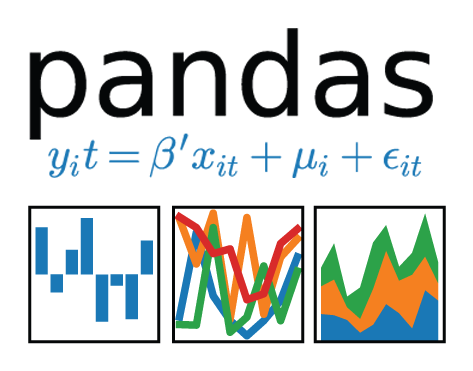
\includegraphics[scale=0.4]{./img/pandas-logo.png}
        \caption{Logo pandas}
        %        \label{}
    \end{figure}

    Pandas to biblioteka napisana w Pythonie służąca do manipulacji i analizy danych.
    Oferuje struktury danych, które ułatwiają operowanie na plikach csv, json i xlsx.
    Umożliwia operacje podobne do znanych z języka SQL.
    Są to: grupowanie danych, sortowanie po indeksie lub po innej kolumnie, łączenie tabel i usuwanie duplikatów.

    \section{git}

    \chapter{Sieć neuronowa}

    \section{Wprowadzenie}

    Sztuczna sieć neuronowa to pewna struktura matematyczna, która może być zaimplementowana programowo lub sprzętowo.
    Początkowo taki twórcy takich modeli inspirowali się zwierzęcym mózgiem, w którym połączone ze sobą neurony tworzą sieć.
    Taka sieć przetwarza sygnały wejściowe wykonując na nich pewne operacje.
    Sieci wykorzystywane są często do rozwiązywania problemów klasyfikacji, z racji na ich zdolność uczenia.
    Np. potrafią przetwarzać zdjęcia i opisywać, co się na nich znajduje.
    Przed skorzystaniem z sieci należy ją nauczyć, co sprowadza się do przekazywania na wejście sieci danych uczących razem z poprawną klasą, do której dane obiekty należą.

    \section{Neuron}

    \begin{figure}[h!]
        \centering
        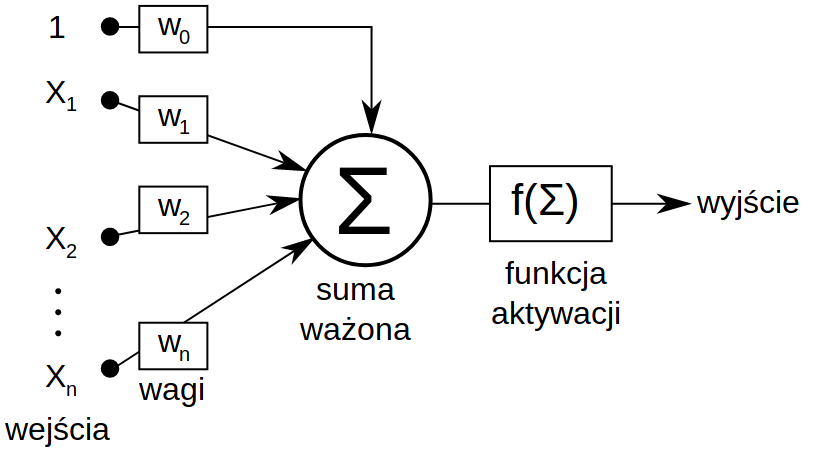
\includegraphics[scale=0.4]{./img/neuron.png}
        \caption{Schemat neuronu}
        %        \label{}
    \end{figure}

    Neuron stanowi podstawowy budulec sztucznej sieci neuronowej.
    Składa się z ustalonej liczby wejść, wraz z odpowiadającymi im wagami.
    Ponadto neuron zawiera nieliniową funkcję aktywacji oraz jedno wyjście.
    Jego zadanie to obliczenie iloczynu skalarnego wektora wejść z wektorem wag.
    Dodatkowo możemy przyjąć, że bias jest dodatkowym wejściem neuronu o wartości 1.
    Następnie obliczona suma ważona poddawana jest funkcji aktywacji i przekazywana na wyjście neuronu.
    W procesie uczenia wagi w neuronie zmieniają się tak, by wyliczona wartość funkcji błędu była jak najmniejsza.

    \subsection{Funkcja aktywacji}

    Funkcja aktywacji to funkcja, która wykorzystywana jest w sztucznych sieciach neuronowych, a dokładniej w samym neuronie do zmiany wartości wyjścia.
    Ma to na celu sprawienie, że sieć jest w stanie lepiej się uczyć nawet przy małej liczby neuronów.
    W uczeniu maszynowym znanych jest wiele rodzajów takich funkcji.
    W tej pracy opiszę tylko dwie, które użyłem do budowy sieci neuronowej.

    \subsubsection{Sigmoid}

    Pierwszą opisywaną funkcją jest sigmoid, zwana też 'sigmoidalną funkcją unipolarną'.
    Bardzo dobrze nadaje się jako funkcja aktywacji, gdyż jej dziedzina to cały zbiór liczb rzeczywistych.
    Ma tę cechę, że zbiór warości mieści się w zakresie (0, 1).
    Jest to również wada, że szybko się 'nasyca'.
    Kolejnym minusem tej funkcji jest to, że wartości nie zcentralizowane wokół zera.
    Ponadto wykorzystuje funkcję ekpotencjalną, która jest kosztowna obliczeniowo.
    Jej wzór to:
    $$
    \sigma(x) = \frac {1}{1+e^{-x}}
    $$

    \begin{figure}[h!]
        \centering
        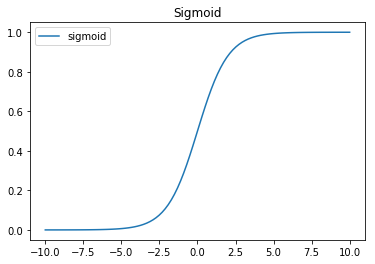
\includegraphics[scale=0.7]{./img/sigmoid.png}
        \caption{Funkcja aktywacji - sigmoid}
        %        \label{}
    \end{figure}

    \subsubsection{Tangens hiperboliczny}
    Kolejna funkcja, która wykorzystywana jest w sieciach neuronowych to tangens hiperboliczny (tanh).
    W tym przypadku również dziedziną jest zbiór liczb rzeczywistych.
    Spłaszcza wyjście w zakresie (-1, 1).
    Podobnie jak sigmoid szybko się 'nasyca'.
    W przeciwieństwie do poprzedniej funkcji jest scentralizowany wokół zera.
    Tanh również korzysta z funkcji ekpotencjalnej.
    Jej wzór to:
    $$
    tanh(x) = \frac {2}{1+e^{-2x}} - 1
    $$

    \begin{figure}[h!]
        \centering
        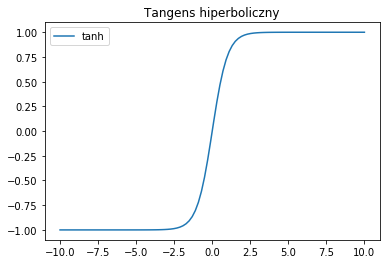
\includegraphics[scale=0.7]{./img/tanh.png}
        \caption{Funkcja aktywacji - tanh}
        %        \label{}
    \end{figure}

    \section{Model wielowarstwowy}

    Kiedy pojedyncze neurony mają te same sygnały wejściowe, tworzą wówczas tak zwaną warstwę w sieci neuronowej.
    Dlatego sieć neuronowa ma budowę warstwową.
    Zawsze występuje warstwa wejściowa i wyjściowa.
    Ponadto mogą występować warstwy ukryte.
    Ich ilość zależy od rozwiązywanego problemu.

    \begin{figure}[h!]
        \centering
        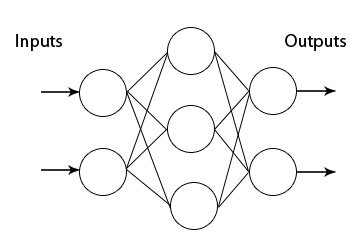
\includegraphics[scale=0.9]{./img/mlp.jpg}
        \caption{Schemat neuronu}
        %        \label{}
    \end{figure}

    W warstwie wejściowej znajduje się tyle neuronów, ile jest badanych cech.
    W moim przypadku będzie mniej niż 31.
    Neurony w tej warstwie nie mają wag, lecz przekazują dalej dokładnie to, co otrzymały.

    Liczba neuronów w warstwie wyjściowej również nie jest przypadkowa.
    Warstwa ta składa się z takiej samej liczby neuronów, co liczba klas w zadanym problemie.
    Problem medyczny, na którym pracuję dotyczy klasyfikacji ośmio klasowej, dlatego będzie osiem neuronów wyjściowych.
    Każdy z nich będzie zwracał wartość przynależności do danej klasy.


    \chapter{Opis architektury aplikacji}

    \section{Schemat warstwy}

    \begin{lstlisting}
        class Layer:
        def __init__(self, shape, activation='sigmoid'):
        ...

        def feedforward(self, x: np.ndarray) -> np.ndarray:
        ...

        def calc_delta(self, d: np.ndarray = None):
        ...

        def calc_gradient(self):
        ...

        def update_weights(self, learning_rate=.2):
        ...
    \end{lstlisting}
    \label{Schemat klasy Layer}

    Powyższy fragment kodu przedstawia schemat klasy Layer.
    Jest to implementacja jednej warstwy w sieci neuronowej.
    Przypomina schemat struktury danych zwanej listą dwukierunkową, gdyż zawiera referencje do poprzedniej i następnej warstwy.
    Klasa zawiera w sobie tablicę, która jest składa się z wag połączeń do poprzedniej warstwy.

    Przy tworzeniu instancji należy podać krotkę liczba oznaczającą kształt warstwy.
    Dodatkowo można przekazać nazwę funkcji aktywacji, którą domyślnie jest to sigmoid.

    Zadanie funkcji 'feedforward' to przyjęcie tablicy liczb z poprzedniej warstwy, obliczenie iloczynu skalarnego z aktualnymi wagami i poddanie wyjścia funkcją aktywacji.
    Następnie funkcja powinna rekurencyjnie wywołać samą siebie na następnej warstwie jeśli nie jest ostatnia w sieci.
    W przeciwnym przypadku zwraca wyliczone wyjście całej sieci.

    Funkcja 'calc\_delta' wywoływana jest rekurencyjne, ale w przeciwnym kierunku.
    Oblicza ona różnicę pomiędzy spodziewanym wyjściem warstwy a aktualnym.
    Pozwoli to później skorygować wagi każdej warstwy.

    Następna funkcja to 'calc\_gradient'.
    Jest równnież wywoływana rekurencyjnie zaczynając od końca sieci.
    Oblicza wartość gradientu na podstawie wyjścia warstwy oraz wartości delty.

    Ostatnią funkcją jest 'update\_weights'.
    Jak jej nazwa wskazuje, to właśnie ona zmienia wartości wag w warstwach odejmując iloczyn obliczonego gradientu ze współczynnikiem uczenia.
    W miarę uczenia współczynnik uczenia może się zmieniać, dlatego uznałem, że to dobre miejsce na dostarczenie tego współczynnika warstwie sieci neuronowej.


    \section{Schemat modelu}

    \subsection{Proces uczenia}

    \chapter{Przeprowadzone badania}

    \chapter{Podsumowanie}

    \section{Dalsze możliwości rozwoju}

    \section{Co mogłem zrobić lepiej}

    Tekst podsumowania

    \bibliography{./bibliography}
    \bibliographystyle{plain}

    \listoffigures
    \listoftables

\end{document}
